\documentclass[book.tex]{subfiles}
\begin{document}
\section{Programming}



Development was done with Borland C++ 3.1 (but the language used was C) which by default ran in EGA mode 3 offering a screen 80 characters wide and 25 characters tall.\\
\par
John Carmack took care of the runtime code. John Romero programmed many of the tools (TED5 map editor, IGRAB asset packer, MUSE sound packer). Jason Blochowiak wrote important subsystems of the game (Input manager, Sound manager, User manager).\\
\par
Borland's solution was an all-in-one package. The IDE, \cw{BC.EXE}, despite some instabilities allowed crude multi-windows code editing with pleasant syntax highlights. The compiler and linker were also part of the package under \cw{BCC.EXE} and \cw{TLINK.EXE}\footnote{Source: Borland C++ 3.1 User Guide.}.\\

\begin{figure}[H]
\centering
  \fullimage{compiling.png}
\caption{Borland C++ 3.1 editor}
\end{figure}
\par

\pagebreak


There was no need to enter command-line mode however. The IDE allowed to create a project, build, run and debug.\\
\par
\begin{figure}[H]
\centering
  \fullimage{borland_compile.png}
  \caption{Compiling Keen Dreams with Borland C++ 3.1}
\end{figure}






Another way to improve screen real estate was to use "high resolution" 50x80 text mode.\\
\par 
 \fullimage{borland_ide_select.png}\\
 \par
 \vspace{-7pt}
The comments still fit perfectly on screen since only the vertical resolution is doubled.\\
\par
\vspace{-4pt}
 \fullimage{borland_ide_highres.png} 
 The file \cw{KD\_MAIN.C} opened in both modes demonstrates the readability/visibility trade-off.\\
\par

  \fullimage{borland_ide_main_lowres.png}\\
\vspace{-5pt}  
   %\vspace{-4pt}
\par
\vspace{5pt}
 \fullimage{borland_ide_main_highres.png}
\section{Graphic Assets}

All graphic assets were produced by Adrian Carmack. All of the work was done with Deluxe Paint (by Brent Iverson, Electronic Arts) and saved in ILBM\footnote{InterLeaved BitMap.} files (Deluxe Paint proprietary format). All assets were hand drawn with a mouse.

\begin{figure}[H]
  \centering
 \fullimage{deluxe_paint.png}
 \caption{Deluxe Paint was used to draw all assets in the game.}
\end{figure}


\subsection{Assets Workflow}
After the graphic assets were generated, a tool (IGRAB) packed all ILBMs together in an archive and generated a header table file (\cw{KDR}-format) and C header file with asset IDs. The engine references an asset directly by using these IDs.\\
\begin{figure}[H]
\centering
 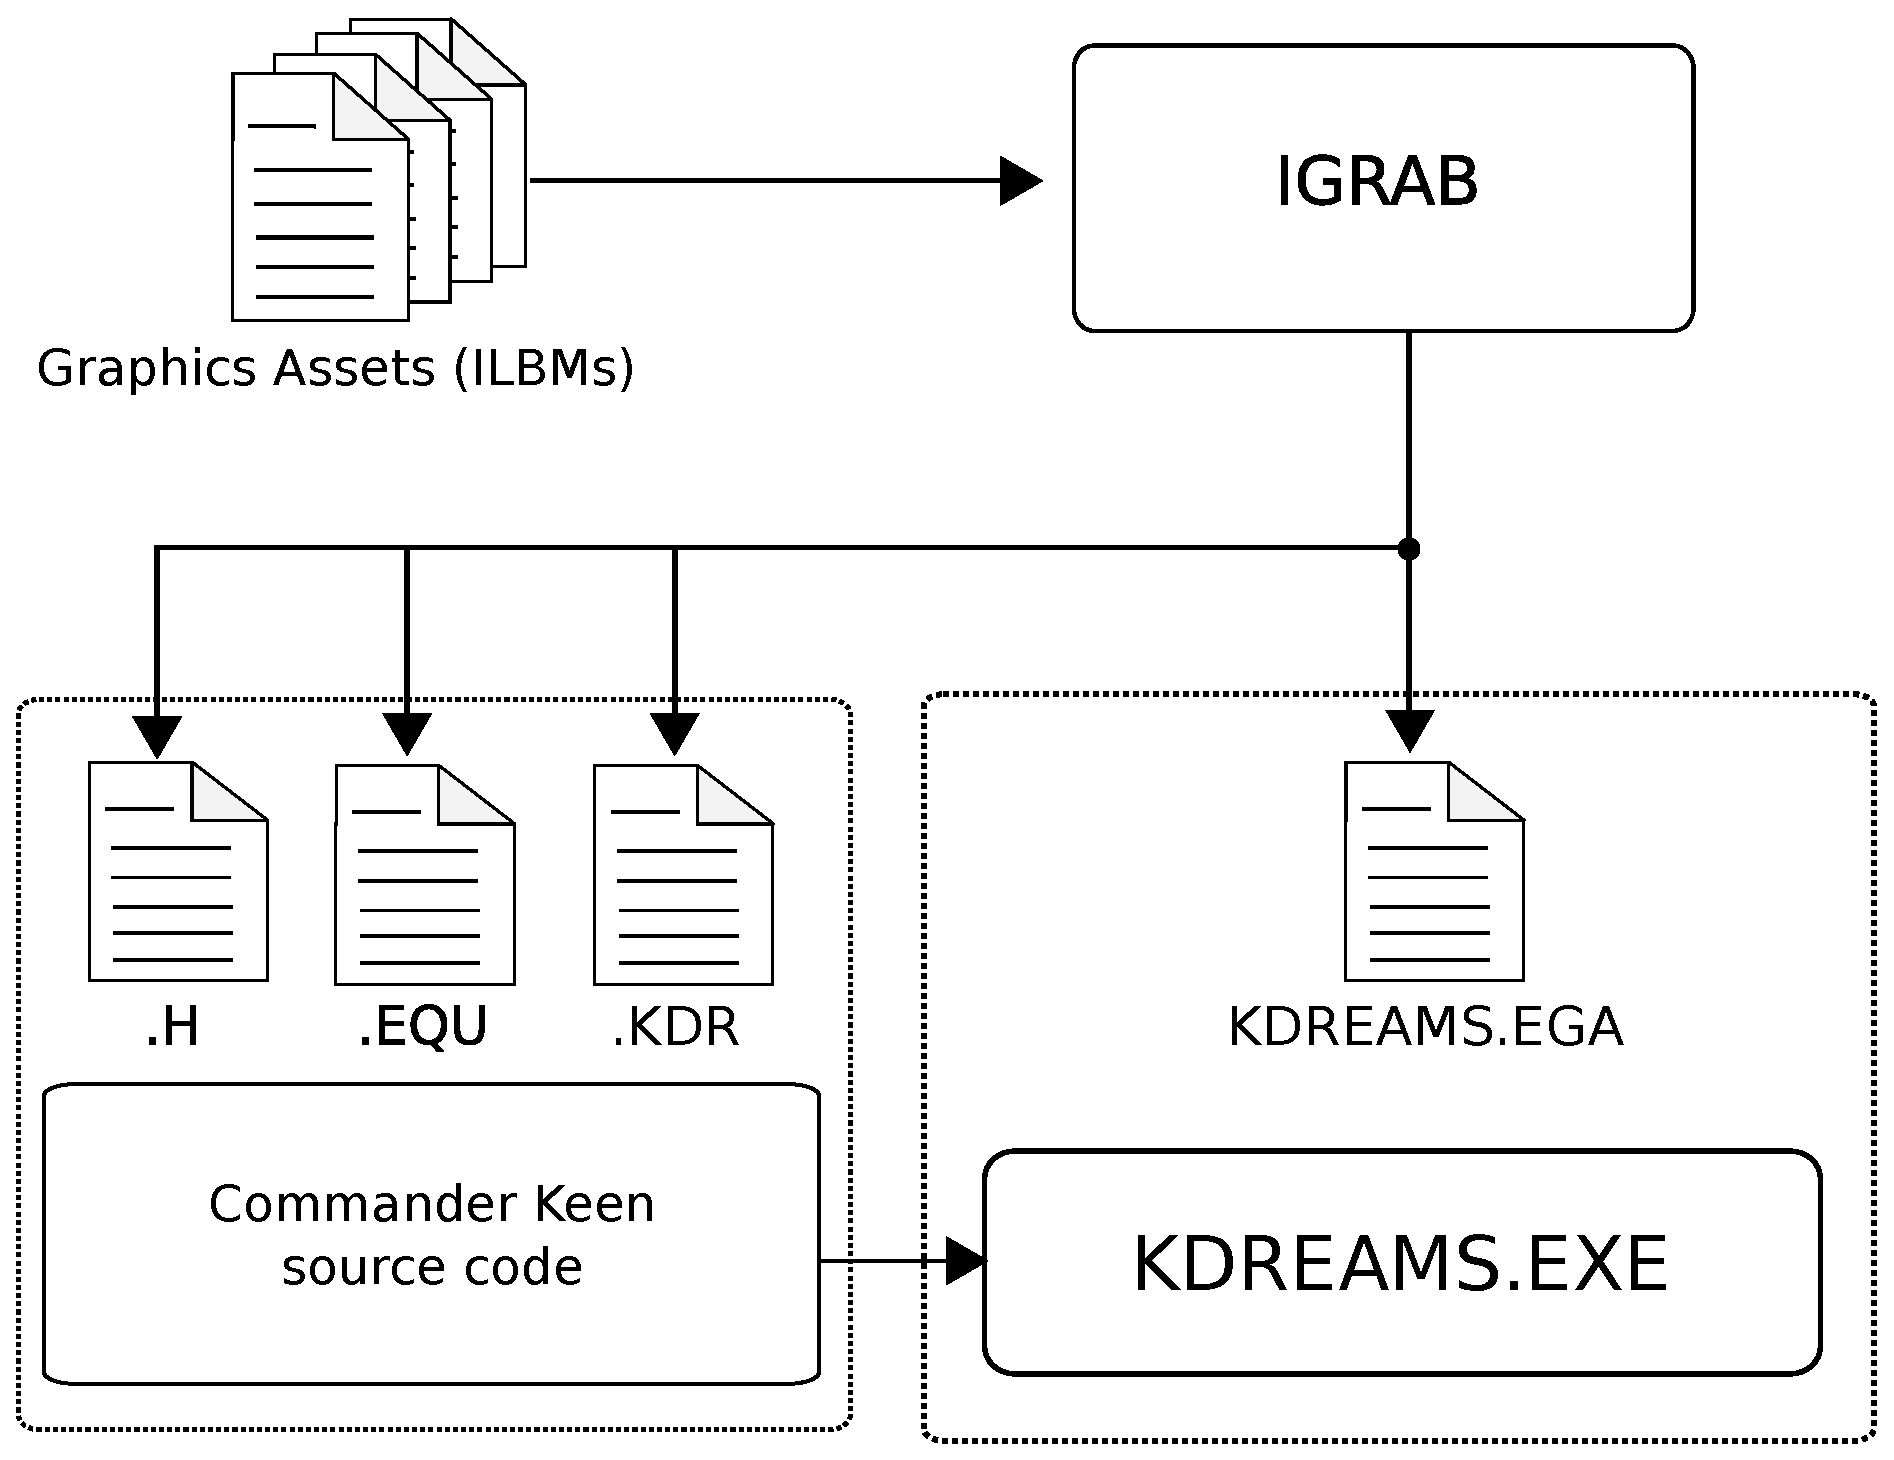
\includegraphics[width=.9\textwidth]{imgs/drawings/drawing_plain.eps}
 \caption{Asset creation pipeline for graphics items}
 \label{asset-creation-pipeline}
\end{figure}
\par
\begin{minipage}{\textwidth}
 \lstinputlisting[language=C]{code/assets_header.c}\par
 \end{minipage}
 
 In the engine code, asset usage is hardcoded via an enum. This enum is an offset into the \cw{HEAD} table which gives an offset in the \cw{DATA} archive. The \cw{HEAD} table files are stored in the \cw{\textbackslash static} folder as \cw{*.KDR} files.\\

\subsection{Assets file structure}
Figure \ref{fig:asset-file} shows the structure of the \cw{KDREAMS.EGA} asset file.
\begin{figure}[H]
\centering
 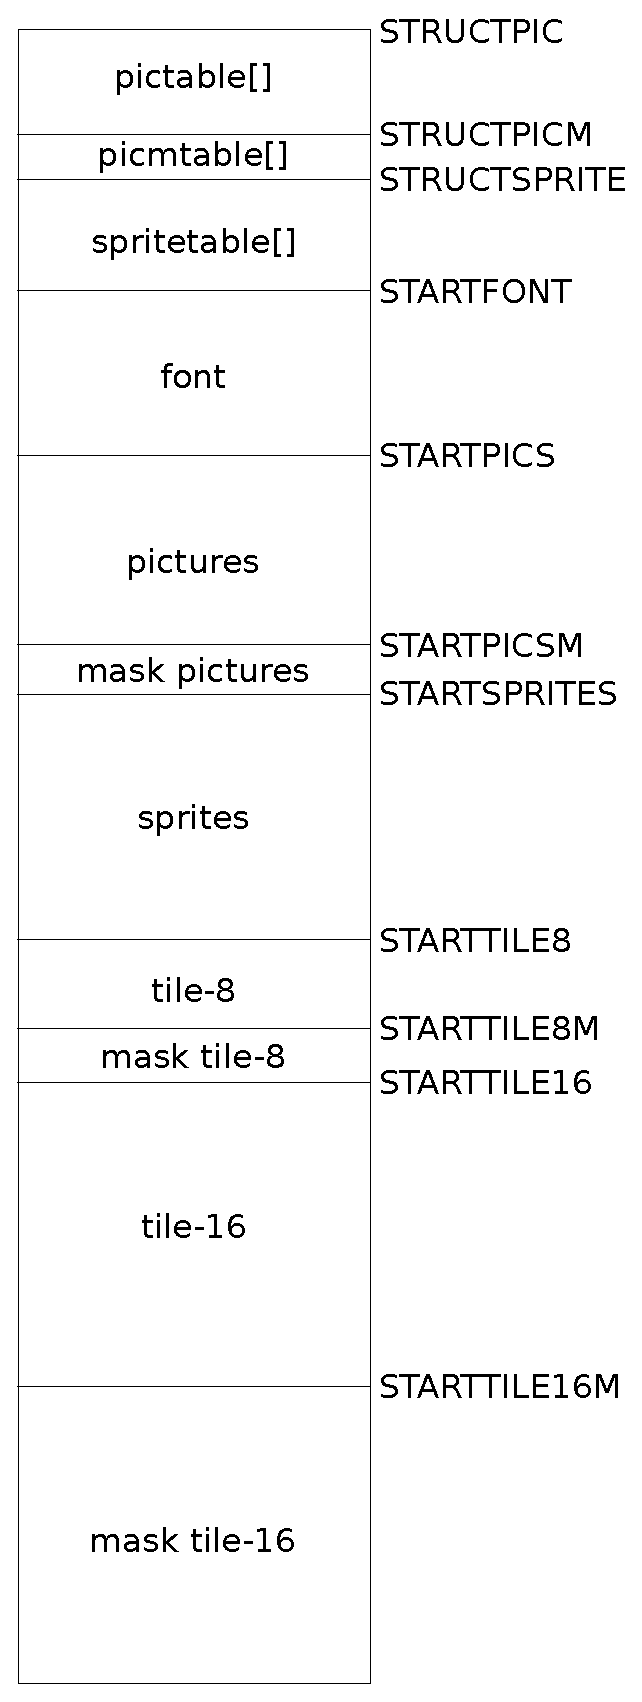
\includegraphics[width=.5\textwidth]{imgs/drawings/graphic_assets.eps}
 \caption{File structure of \cw{KDREAMS.EGA} asset file.}
 \label{fig:asset-file}
\end{figure}

The \cw{pictable[]} contains the width and height in bytes for each picture in the asset file. Note that a width of 5 bytes means a size of 40 pixels on the screen. The same size structure is applied for mask pictures.\\

  \begin{table}[H]
  \begin{tabularx}{0.8\textwidth}[c]{XXX}
  \hline
  \textbf{index} & \textbf{width} & \textbf{height}   \\ \hline
  0             & 5          & 32    \\
  1             & 5          & 32    \\
  2             & 5          & 32    \\
  3             & 5          & 32    \\
  4             & 5          & 32    \\
  5             & 5          & 32    \\
  6             & 5          & 32    \\
  7             & 5          & 32    \\
  ...             & ...          & ...    \\
  64             & 5          & 24    \\
  \end{tabularx}
  \caption{content of pictable[].}
  \end{table}



The \cw{spritetable[]} contains beside width and height in bytes also information on the sprite center, hit boundaries and number of shifted sprites (this will be explained in section xxx). \\

\begin{table}[H]
  \begin{tabularx}{\textwidth}[c]{lXXXXXXXXX}
  \hline
  \textbf{index} & \textbf{width} & \textbf{height} & \textbf{orgx} & \textbf{orgy}
    & \textbf{xl} & \textbf{yl} & \textbf{xh} & \textbf{yh} & \textbf{shift} \\ \hline
  0  &   3  &   24  &   0  &   0  &   0  &   0  &   368  &   368  &   4 \\
  1  &   3  &   32  &   0  &   0  &   64  &   0  &   304  &   496  &   4 \\
  2  &   3  &   30  &   0  &   16  &   64  &   0  &   304  &   496  &   4 \\
  3  &   3  &   30  &   0  &   32  &   64  &   48  &   304  &   496  &   4 \\
  4  &   3  &   32  &   0  &   0  &   64  &   0  &   304  &   496  &   4 \\
  5  &   3  &   30  &   0  &   32  &   64  &   48  &   304  &   496  &   4 \\
 ...  &   ...  &   ...  &   ...  &   ...  &   ...  &   ...  &   ...  &   ...  &   ... \\
 296  &   12  &   103  &   -128  &   0  &   256  &   128  &   752  &   1648  &   4\\
  \end{tabularx}
  \caption{content of spritetable[].}
  \end{table}

The font segment contains a table for the height (same for all characters) and width of the font, as well as a reference where the character data is located.\\
\par
\begin{minipage}{\textwidth}
 \lstinputlisting[language=C]{code/font_structure.c}\par
 \end{minipage}
\begin{figure}[H] 
  \centering 
  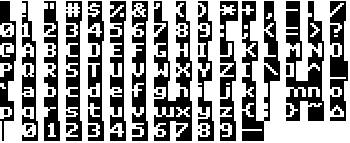
\includegraphics[width=1.0\textwidth, frame]{screenshots_300dpi/font.png}
  \caption{Font assets data.}
  \label{fig:font_assets}
\end{figure} 

Since all tiles have fixed dimension (either 8 or 16 pixels), there is no need to store any tile size table structure. From \cw{STARTPICS} location onwards all graphical assets are stored. Each asset contains four planes, aligned with the EGA architecture. Foreground tiles and sprites include a mask plane as well.
 
\begin{figure}[H] 
  \centering 
  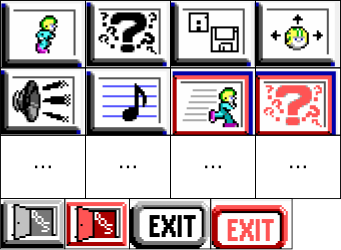
\includegraphics[width=1.0\textwidth, frame]{screenshots_300dpi/pics_assets.png}
  \caption{Picture assets data.}
  \label{fig:picture_assets}
\end{figure} 

\begin{figure}[H] 
  \centering 
  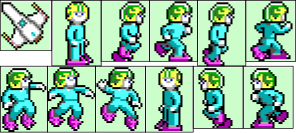
\includegraphics[width=1.0\textwidth, frame]{screenshots_300dpi/sprite_assets.png}
  \caption{Sprite assets data.}
  \label{fig:sprite_assets}
\end{figure} 

\begin{figure}[H] 
  \centering 
  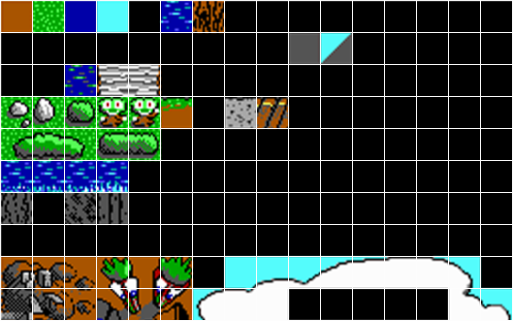
\includegraphics[width=0.9\textwidth, frame]{screenshots_300dpi/tile16_assets.png}
\end{figure} 

\begin{figure}[H] 
  \centering 
  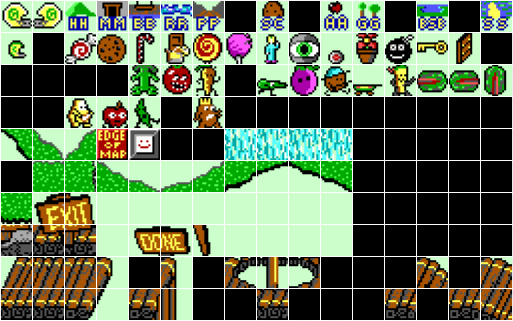
\includegraphics[width=0.9\textwidth, frame]{screenshots_300dpi/tile16M_assets.png}
  \caption{Background (Tile-16) and foreground (masked tile-16) assets data.}
  \label{fig:tile16_assets}
\end{figure} 



\section{Maps}
Maps were created using an in-house editor called TED5, short for Tile EDitor. Over the years TED5 had improvements and the same tool is used for creating maps of both side-scrolling games and top-down games like Wolf 3D.\\
\par
 TED5 is not stand-alone; in order to start, it needs an asset archive and the  associated header (as described in the graphic asset workflow Figure \ref{asset-creation-pipeline} on page \pageref{asset-creation-pipeline}). This way, texture IDs are directly encoded in the map.\\

 
 \fullimage{TedSplashscreen.png}
 \par
 \trivia{The suffix, "vD.IP", was put in by the Rise of the Triad team in 1994. It stood for "Developers of Incredible Power".}\\
 \par
\fullimage{Fill_2.png}\\
 


 \fullimage{ted5_scrolling_map.png}\\
\par



 \par
 TED5 allows placement of tiles on layers called "planes". In Commander Keen, layers are used for background, foreground and information tiles. Note that foreground tiles are always using a mask as they are overlayed with the background. The info plane contains the location of all actors and special places. Each foreground and background tile could also be enriched with additional tile information such as tile clipping and tile animations. Just like IGRAB, the TED5 tool generated a header table file (\cw{KDR}-format) and a \cw{*.MAP} file containing the levels. Figure \ref{fig:map-header-file} shows the map header table, which is hard-coded in the source code.
\begin{figure}[H]
\centering
 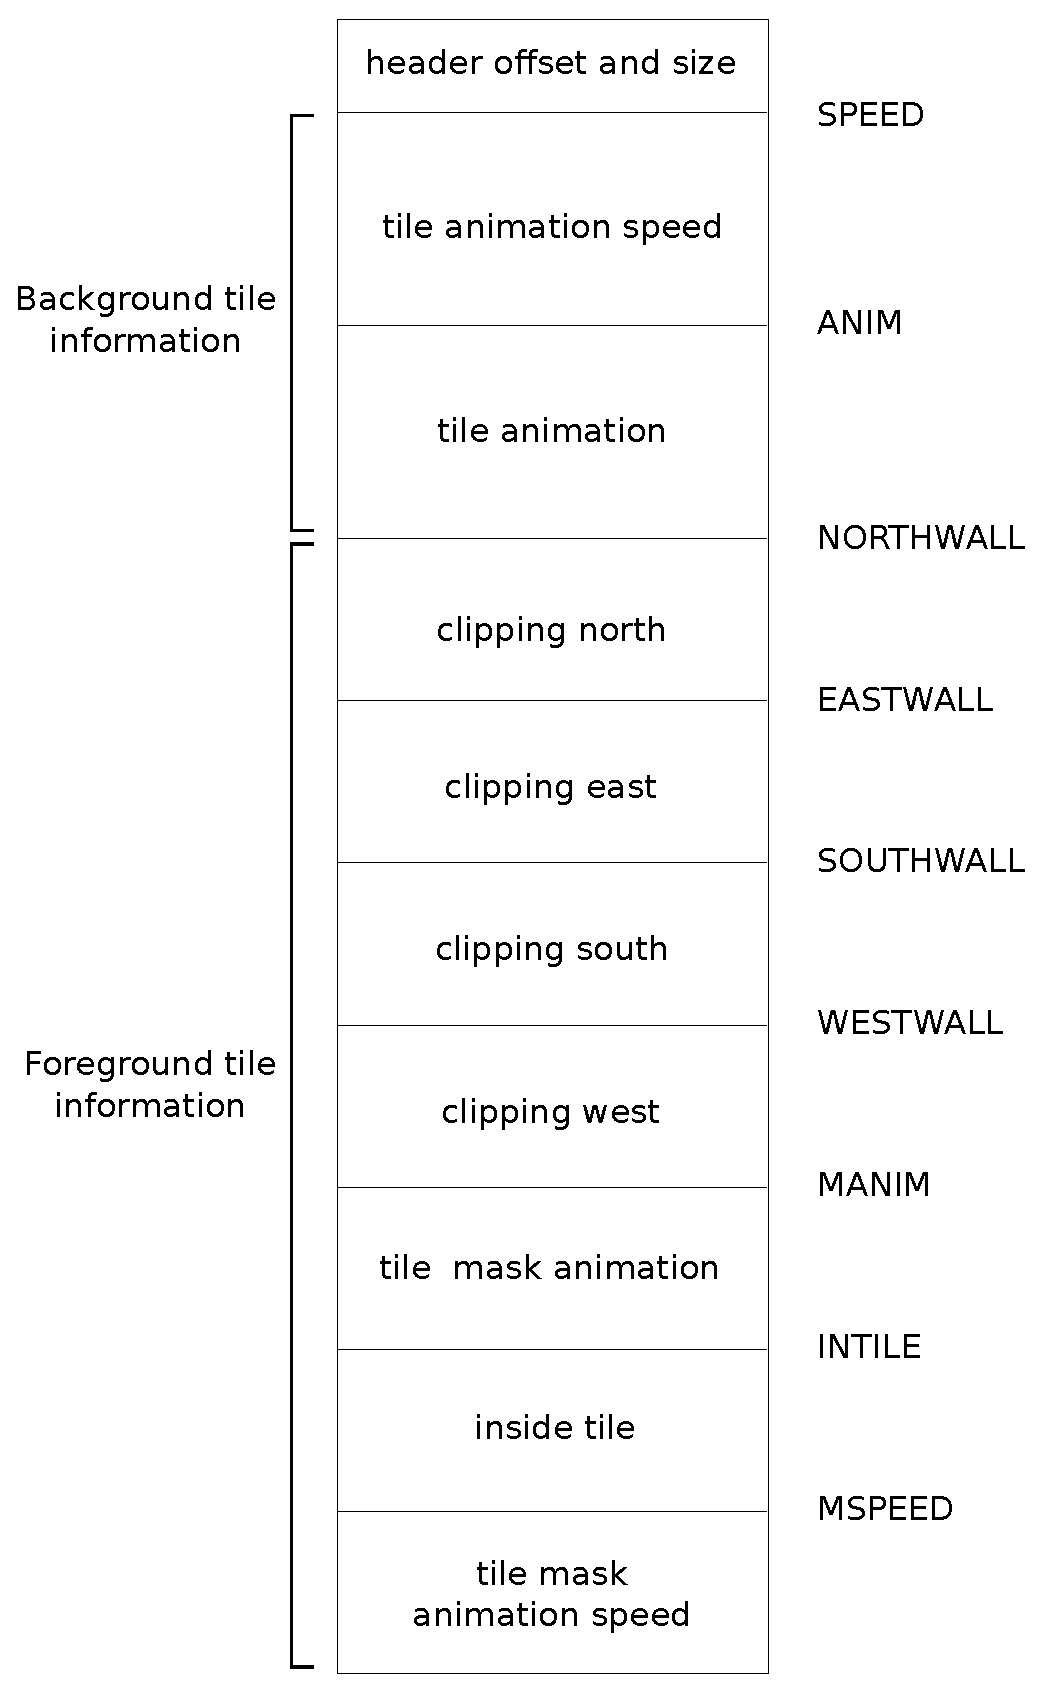
\includegraphics[width=.7\textwidth]{imgs/drawings/map_header.eps}
 \caption{File structure of \cw{MAPHEAD.KDR} header file.}
 \label{fig:map-header-file}
\end{figure}

\subsection{Map header structure}
The header offset and header size refer to the location and size in the \cw{KDREAMS.MAP} file. A total of 100 maps are supported in the game.\\
\par
\begin{minipage}{\textwidth}
 \lstinputlisting[language=C]{code/map_header_structure.c}\par
 \end{minipage}

\subsection{Background tile information}
For background tile animation two information tables are required: tile animation and tile animation speed. The tile animation refers to the next tile in the animation sequence. So in case of tile \#90, the next animation tile is \#91 (+1), followed by \#92 (+1) and \#93 (+1). After tile \#93 (-3) the sequence is going back to tile \#90. The animation speed is expressed in TimeCount, which is the number of ticks before the next tile is displayed. \\
 \begin{table}[H]
  \begin{tabularx}{\textwidth}[c]{XXX}
  \hline
  \textbf{index} & \textbf{tile animation} & \textbf{tile animation speed}   \\ \hline
  0             & 0          & 0    \\
  1             & 0          & 0    \\
  ...             & ...          & ...    \\
  57             & 1          & 32    \\
  58             & -1          & 24    \\
  ...             & ...          & ...    \\
  90             & 1          & 8    \\
  91            & 1          & 8    \\
  92             & 1          & 8    \\
  93             & -3          & 8    \\
  ...             & ...          & ...    \\
  \end{tabularx}
  \caption{Background tile animation.}
  \end{table}

\subsection{Foreground tile information}
The foreground tiles contain some additional information tables. Beside tile animation (tile mask animation and tile mask animation speed, similar like background tiles) it also contains clipping and 'inside' tile information.\\
\par
The clipping tables contains how Commander Keen is clipped against foreground tiles. 'Inside' tile information is used to climb on a pole and illustrate Commander Keen is going through a floor opening ('inside' the tile). In section \ref{section:clipping} both the clipping and 'inside' logic is further explained.\\
\begin{table}[H]
  \begin{tabularx}{\textwidth}[c]{XXXXXXX}
  \hline
  \textbf{index} & \textbf{clip north} & \textbf{clip east} & \textbf{clip south} & \textbf{clip west}  & \textbf{inside tile} \\ \hline
  ...    & ...     & ...    & ...   & ...     & ...      \\
  238    & 0       & 1      & 5     & 0       & 0        \\
  239    & 0       & 0      & 0     & 0       & 0        \\
  240    & 0       & 0      & 5     & 0       & 0        \\
  241    & 0       & 0      & 0     & 0       & 128       \\
  242    & 1       & 1      & 1     & 1       & 128       \\
  243    & 1       & 0      & 1     & 0       & 0       \\
  244    & 0       & 0      & 2     & 0       & 0       \\
  ...    & ...     & ...    & ...   & ...     & ...     \\
  \end{tabularx}
  \caption{Foreground tile clipping and 'inside' tile information.}
  \end{table}










The size of each tile information block is defined by the amount of tile-16 and mask tile-16 data items in the IGRAB tool.\\
\par
\begin{minipage}{\textwidth}
 \lstinputlisting[language=C]{code/map_header.c}\par
 \end{minipage}
 
 
\subsection{Map file structure}
The structure of \cw{KDREAMS.MAP} is explain in Figure \ref{fig:map-file}. For each map there is a small header containing the width, height and name of the map as well as a reference pointer to each of the three planes. Each plane exists out of a map of tile numbers for foreground, background and info.
\begin{figure}[H]
\centering
 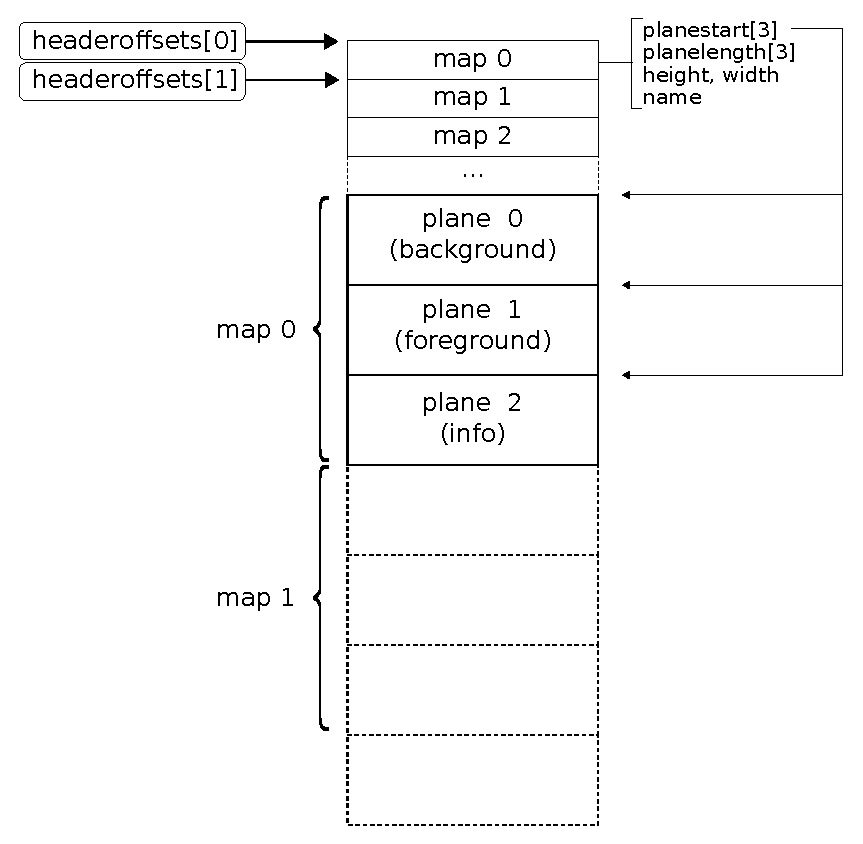
\includegraphics[width=\textwidth]{imgs/drawings/kdreams_map.eps}
 \caption{File structure of \cw{KDREAMS.MAP} file.}
 \label{fig:map-file}
\end{figure}

\end{document}
